\chapter{État de l'art sur l'Internet des Objets}
\label{chap:etat-art}

\paragraph{} Comme dit dans l'introduction, Libelium est notre fournisseur de matériel. Cela s'explique par le fait qu'un groupe précédent d'étudiants a déjà fait un projet à l'aide de ces capteurs il y a 2 ans; nous avons donc continué avec ce même matériel. Dans cette partie, nous voyons quelles offres Libelium propose en matière d'IoT ainsi qu'une comparaison entre les différentes technologies utilisées. 

\section{Comparaison des différents protocoles}
    \paragraph{}Libelium présente un très grand panel d'outils et de produits pour répondre aux besoins de l'IoT. Ils proposent des très nombreux capteurs, du plus habituel (capteur de température) au plus spécifique (compteur Geiger par exemple). Ils vendent également de nombreux packs adaptés (packs pour les milieux aquatiques, pour l'agriculture, pour des \emph{Smart City}, pour la sécurité, \dots) et des solutions pour centraliser la récolte de données en un appareil et l'envoyer vers un serveur par exemple. On trouve également des packs plus simples et plus généraux. L'entreprise dispose également de services \emph{cloud}, permettant de déléguer la partie serveur, hébergement et stockage de données à son infrastructure.\\
    La pierre angulaire de la plupart des solutions est une carte de développement appelée Waspmote disposant d'un microcontrôleur et qui permet de brancher de nombreux capteurs et/ou cartes d'extension.

    \paragraph{} Ces Waspmotes peuvent communiquer entre elles ou avec d'autres réseaux en utilisant divers protocoles. Nous allons présenter ces différents protocoles, leurs avantages, leurs inconvénients pour les comparer. La figure \ref{tab:ondes} présente les différents modules de communication compatibles avec les Waspmotes. 
    
    \paragraph{} Les différents modules peuvent être classés en deux catégories : ceux qui ont un débit conséquent et les autres. Les technologies mobiles (GPRS/3G/4G) et le Wi-Fi proposent des débits intéressants mais consomment beaucoup trop d'énergie dans un contexte de cartes et capteurs isolés et alimentés par batterie. Le module GPRS/3G peut néanmoins être utile : il consomme moins d'énergie que les autres modules utilisant des technologies mobiles et permet d'envoyer des données depuis un endroit isolé.

    \begin{table}[h]
        \centering
        \begin{tabular}{C{2.7cm} | C{2.4cm} | C{2.6cm} | C{2.3cm} | C{2cm} | C{1.7cm}}
            \textbf{Module}			    		&	\textbf{Nb}\tabularnewline\hline
Waspmote 802.15.4 PRO           	&   6\tabularnewline
Waspmote Gateway 802.15.4       	&   2\tabularnewline
GPS Module                      	&   1\tabularnewline
GSM / GPRS Module					&	1\tabularnewline
3G + GPS Module						&	1\tabularnewline
Bluetooth							&	1\tabularnewline
Bluetooth Module PRO 5 dBi			&	1\tabularnewline
Waspmote RFID 13.56 MHz				&	1\tabularnewline
5 NFC stickers                      &	1\tabularnewline
WiFi module 5 dBi					&	1\tabularnewline

        \end{tabular}
        \caption{Spécifications théoriques des différents modules de communication}
        \label{tab:ondes}
    \end{table}

    
    \paragraph{}L'IoT se développe principalement avec les autres types de modules et de protocoles qui ont été pensés pour ne pas dépenser trop d'énergie afin d'assurer une autonomie importante. De plus, les données envoyées par les capteurs ne sont généralement pas très lourdes et peuvent donc se contenter de débit faible (voir très faible). On retrouve dans cette catégorie le \textbf{Sigfox}, \textbf{LoRaWan}\footnote{LoRaWAN pour Long Range Wide-area network}, \textbf{Zigbee} et le \textbf{Bluetooth Low Energy (BLE)}.

    \paragraph{}Le \textbf{Sigfox} est une technologie développée en France qui se différencie de ses concurrentes par son modèle économique. C'est une sorte d'opérateur téléphonique mais pour l'IoT. L'utilisateur paie donc un abonnement pour pouvoir accéder au réseau Sigfox basse consommation et communiquer comme le ferait un appareil mobile sur un réseau 3G/4G. Sigfox désigne à la fois un protocole de communication, un réseau IoT et un opérateur IoT. Le protocole de communication permet des débits très faibles, suffisants pour des données simples (comme la température) mais qui peuvent devenir rapidement limitant. La couverture Sigfox en France (et plus généralement en Europe de l'Ouest) est très bonne. Ce protocole est plutôt utilisé pour disposer des capteurs sur des zones de plusieurs km² puisque chaque carte comportant le module Sigfox peut communiquer sur le réseau Sigfox. Celui-ci est relié à Internet et permet donc d'envoyer les données sur un serveur distant.

    \paragraph{}\textbf{LoRaWAN} est un protocole de communication radio bas débit et basse consommation. Les réseaux LoRaWAN sont en étoile, les Waspmotes comportant des capteurs communiquent avec un dispositif central chargé d'assumer le rôle de passerelle entre les Wasmpotes et le serveur.  C'est le protocole le plus efficace en terme de consommation d'énergie, une Waspmote pouvant rester jusqu'à 6 ans sans rechargement de batterie dans des conditions d'utilisation normales. Cette technologie autorise des débits allant jusqu'à 50 kbit/s et une portée théorique de plusieurs kilomètres (5km en urbain, 15 km ailleurs)

    \paragraph{}Le \textbf{Zigbee} (ou protocole 802.15.4 dans le tableau \ref{tab:ondes}) est un protocole ouvert très similaire à LoRaWAN. Il autorise des débits plus importants (de l'ordre de 250 kbit/s) mais ne garantit qu'une portée beaucoup plus inférieure (plusieurs centaines de mètres en théorie, plutôt aux environs de 7 à 10m dans les faits d'après nos tests). Son avantage consiste dans la modularité de ses configurations réseaux : il est possible de faire un réseau en étoile avec un dispositif central, comme avec LoRaWAN, mais aussi un réseau maillé où chaque Waspmote est en mesure de communiquer avec toutes ses voisines et de transmettre les informations de pair à pair. La consommation reste très basse mais est supérieure à celle de LoRaWAN.

    \paragraph{} Le \textbf{BLE}  est une norme du Bluetooth spécialement pensée pour l'IoT, très proche en caractéristiques du Zigbee. La portée et la consommation sont similaires au Zigbee, mais avec un débit 4 fois plus élevé (1 Mbit/s contre 250 kbit/s pour Zigbee). C'est un protocole qui se retrouve énormément dans la téléphonie mobile et avec le développement d'objets contrôlables par Smartphone. C'est donc un protocole qui est utilisé dans une autre branche de l'IoT, comparé à LoRaWAN ou Zigbee qui sont plutôt spécialisés dans des travaux scientifiques ou l'aménagement et la supervision du territoire. Cependant, le Bluetooth, poussé par sa complémentarité avec les technologies mobiles, est en train de devenir un acteur principal de l'IoT et son évolution est très rapide (5 normes Bluetooth en 10 ans, contre une pour Zigbee et 0 pour LoRa).

\section{Impact des ondes sur la santé des lémuriens} % Peut-être faire un truc sur la pollution lumineuse des capteurs si on a le temps (lol)

    \paragraph{}Ces différentes technologies de communication ont toutes pour point commun leur mode de transmission sans fil. Les différents capteurs étant placés dans les pièces --- voire dans les cages --- où se situent les lémuriens, il est important de savoir comment les ondes électromagnétiques générées par les capteurs peuvent impacter la santé des lémuriens.\\
    Ce potentiel impact des champs électromagnétiques sur les êtres vivants est l'une des questions modernes parmi les plus controversées \cite{INRS} (au même titre que l'impact sanitaire des OGM), en particulier son impact sur la santé humaine. À l'heure actuelle, la communauté scientifique semble s'accorder sur le fait que nous ne disposons pas d'assez de données et que nous manquons de recul pour trancher la question de la nocivité des ondes sur les individus sains (pas de maladie ou de prédispositions génétiques). En particulier, nous n'avons pas trouvé d'étude évaluant l'impact des ondes sur les lémuriens. Néanmoins, nous avons trouvé plusieurs études exposant des expérimentations réalisées sur des souris ou des rats. Les lémuriens \textit{\ref{fig:lemuzob}} et les rats étant tous deux des mammifères de masse similaire, ces études peuvent nous apporter quelques indices bien qu'il faille prendre en compte de nombreux autres facteurs qui nous échappent.
   
    \paragraph{}La première étude \cite{test2} a analysé l'impact des ondes électromagnétiques émises par les téléphones mobiles sur une population de souris atteinte de la maladie d'Alzheimer. Les téléphones mobiles fonctionnent avec des antennes utilisant des fréquences similaires à celles utilisées par les différents protocoles pré-exposés (entre 700~MHz et 3~GHz). Il est donc possible de faire un rapprochement au niveau du type d'onde. Ces souris ont également la maladie d'Alzheimer\cite{BONS1996S66}, point intéressant puisque cette maladie est étudiée en particulier sur notre population de lémuriens. Les résultats de cette étude peuvent être assez surprenants. En effet, les souris ayant développé la maladie d'Alzheimer (elles ont été génétiquement modifiées dans ce but) ont pu retrouver une partie de leurs facultés mentales suite à une exposition régulière aux ondes. Sur de jeunes souris génétiquement modifiées, l'exposition aux ondes a eu semblerait-il un effet préventif : elles n'ont pas développé la maladie alors qu'elles auraient du en temps normal. Les ondes de cette bande de fréquences ont donc semble-t-il régénéré les zones du cerveau attaquées par la maladie d'Alzheimer. Ces résultats ne sont néanmoins que le début, et il est nécessaire de poursuivre les études sur le sujet pour confirmer ou infirmer ces résultats.
    
    \begin{figure}[h]
        \centering
        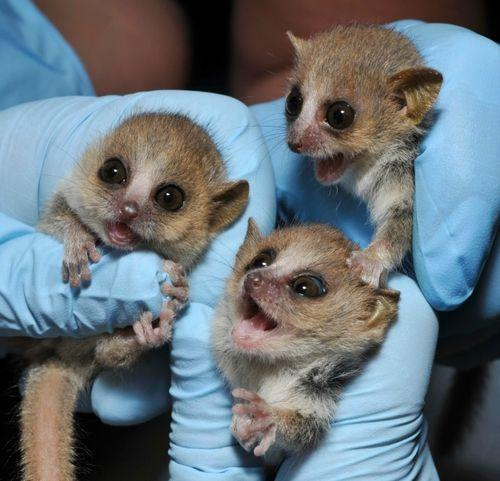
\includegraphics[scale=0.35]{images/photos/lemuzobs.jpg}
        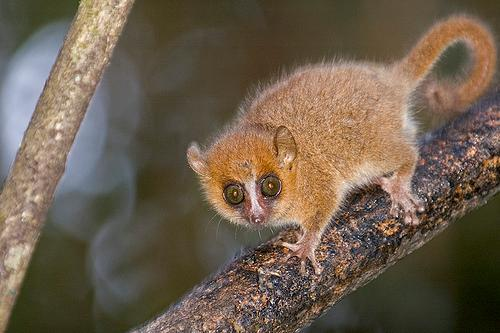
\includegraphics[trim={4.3cm 0cm 0cm 0cm},clip,scale=0.505]{images/photos/lemu.jpg}
        \caption{Photos de lémuriens Microcebus}
        \label{fig:lemuzob}
    \end{figure}
    
    \paragraph{} Nous avons relevé une autre étude  \cite{test1} qui s'intéresse à l'impact des ondes sur la physiologie des rats. Les rats étudiés ont été exposés pendant 5 semaines à une émission continue d'ondes. La fréquence des ondes utilisée est de 900~MHz, soit similaire ---~comme pour l'étude précédente~--- aux technologies de réseau de capteurs. Les chercheurs ont pu arriver à trois résultats :
    
    \begin{enumerate}
        \item Dans un contexte de température assez élevée (31~°C) , les rats exposés ont tendance à avoir certaines parties du corps --- comme la queue --- plus froides (de l'ordre de 1,6~°C). Ce processus se déclenche pour éviter les pertes d'énergie, comme si leurs dépenses étaient en parallèle accrues.
        \item Dans un contexte similaire de chaleur, les rats ont tendance à manger plus, ce que les chercheurs interprètent comme une conséquence du premier point.
        \item Quelle que soit la température ambiante, les rats exposés ont des phases de sommeil paradoxal (phase des rêves) plus nombreuses que les rats témoins, comme s'ils étaient en alerte. Néanmoins cela n'a pas l'air d'impacter la qualité du sommeil des rats exposés aux émissions d'ondes. Tous les animaux dormaient autant et ne manifestaient pas plus de difficultés à trouver le sommeil.
    \end{enumerate}
    Les ondes semblent donc avoir un impact sur la physiologie des rats, mais là encore la recherche n'en est qu'à ses débuts. Il est à noter que l'impact est étudié dans un contexte d'émission continue d'ondes, ce qui ne serait pas forcément le cas pour notre projet.
    
   
    \paragraph{}Enfin la dernière étude relevée est un état de l'art des nombreuses études réalisées sur le sujet \cite{SAY201670}. En effet, de nombreuses équipes de recherche abordent le problème rigoureusement et en viennent à la conclusion qu'il semble exister un lien de causalité entre la présence de champs électromagnétique et les réactions biologiques de la part de certains sujets d'expérimentation. Dans la majorité de ces études, les tests d'exposition ont été réalisés sur différents groupes de sujets, certains étant atteints de faiblesses (maladies diverses),  les autres étant généralement sains. Ces tests aboutissent à la conclusion que si les sujets sains ne semblent pas avoir été impactés, les sujets fragiles --- présentant initialement des faiblesses diverses --- voient leur métabolisme subir diverses modifications.
    
    
    \paragraph{}Les chercheurs s'accordent à dire qu'au vue des connaissances actuelles, les ondes n'ont pas d'impact dangereux. Il est néanmoins possible de constater certains effets (pas nécessairement négatifs, comme vu dans la première étude) dans des conditions d'émission continue, et notamment sur des individus ayant des prédispositions génétiques ou des faiblesses. Ces résultats sont à nuancer dans le cas de notre projet, puisque les capteurs ne seront pas activés et/ou en transmission en permanence. De plus, ils ne seront pas forcément aussi proche des lémuriens que les rats et souris des études citées. Il reste cependant intéressant de prendre ces résultats en considération et d'évaluer le possible impact des ondes sur la santé des lémuriens.




